%=================================================
% Economics Coursework Template
%=================================================
\documentclass[12pt]{article}

%------------ Packages ------------
\usepackage[margin=1in]{geometry}   % Page layout
\usepackage{lmodern}                % Latin Modern (LaTeX default font)
\usepackage{amsmath, amssymb}       % Math symbols
\usepackage{booktabs}               % Professional tables
\usepackage{graphicx}               % Figures
\usepackage{natbib}                 % References
\usepackage[hidelinks]{hyperref}    % Hyperlinks
\usepackage{fancyhdr}               % Headers/footers
\usepackage{setspace}               % Line spacing
\usepackage{titlesec}               % Section formatting
\usepackage{geometry}
\usepackage{comment} 
\usepackage{xcolor} 
\usepackage{amsthm} 
\usepackage{float} 
\usepackage{dcolumn}
\usepackage{titlesec}
\usepackage{enumitem}
\usepackage{hyperref}
\usepackage{tikz}
\usepackage{multicol}
\usetikzlibrary{arrows.meta,positioning,fit,calc}
\usepackage{subcaption}
\tikzset{
  var/.style={rectangle, draw, rounded corners, minimum width=18mm, minimum height=7mm, align=center},
  latent/.style={ellipse, draw, dashed, minimum width=18mm, minimum height=7mm, align=center},
  controlarrow/.style={->, dashed, draw=red!60},
  lightbluearrow/.style={->, dashed, draw=blue!40} % NEW style
}

%------------ Page Style ------------
\rhead{\thepage}
\lhead{ECO1465 Weekly Report 1}

%------------ Section Formatting ------------
\titleformat{\section}{\large\bfseries}{\thesection.}{0.5em}{}
\titleformat{\subsection}{\normalsize\bfseries\itshape}{\thesubsection}{0.5em}{}
\titlespacing*{\subsection}{0pt}{1.5ex plus 1ex minus .2ex}{1em} % spacing before/after subsections


%------------ Begin Document ------------
\begin{document}
% Title Page only
\begin{titlepage}
    \thispagestyle{empty} % no headers/footers
    \centering
    \vspace*{\fill}

    {\Large \textbf{Cournot Competition} \par}

    \vspace{3em}
    {\large Nardeen Abdulkareem \par}
    {\normalsize The University of Toronto \par}
    {\normalsize \today \par}
    {\texttt{nardeen.abdulkareem@mail.utoronto.ca} \par}

    \vspace*{\fill}
\end{titlepage}
\clearpage

\section{Equilibrium Derivation}
\subsection{Strategic Substitutes or Complements?}
$$P_i = \alpha_0 + \alpha_1 q_i + \alpha_1 \sum^N_{j \neq i}q_j + \alpha_2 Y + \eta$$
$$ \pi_i = (\alpha_0 + \alpha_1 q_i + \alpha_1 \sum^N_{j \neq i}q_j + \alpha_2 Y + \eta)q_i - (\gamma_0 + \gamma_1W + \omega_i)q_i - \gamma_2 qi^2$$
$$\frac{\partial \pi_i}{\partial q_i} = (\alpha_0 + \alpha_1 q_i + \alpha_1 \sum^N_{j \neq i}q_j + \alpha_2 Y + \eta) + (\alpha_1 q_i) - (\gamma_0 + \gamma_1W + \omega_i) - 2 \gamma_2 q_i = 0$$
$$q_i =  - \frac{\alpha_0 + \alpha_1 \sum^N_{j \neq i}q_j + \alpha_2 Y + \eta - \gamma_0 - \gamma_1W - \omega_i}{2(\alpha_1 - \gamma_2)} $$
$$\frac{\partial^2 \pi_i}{\partial q_i \partial q_j} = \frac{\partial^2 \pi_i}{\partial q_j \partial q_i} = \alpha_1 \quad \text{where: } \alpha_1 < 1$$

Since the cross partial above is negative, this means that cournot competition yields a game of strategic substitutes. What this really means is that if firm i raises their quantity produced other firms will react by reducing their quantities (since cournot competition is quantity setting game).
$$ \frac{\partial q_i}{\partial q_j} = - \frac{\alpha_1}{2(\alpha_1 - \gamma_2)}$$

Since $\alpha_1 < 0$ and $\gamma_2 > 0$ the $ \frac{\partial q_i}{\partial q_j}$ term is negative which means that with an increase in quantities produced by firm j, firm i will lower it's output produced.

\subsection{Two Firms Case}
$$ \pi_i = (\alpha_0 + \alpha_1 q_i + \alpha_1 q_j + \alpha_2 Y + \eta)q_i - (\gamma_0 + \gamma_1W + \omega_i)q_i - \gamma_2 qi^2$$
$$ \pi_j = (\alpha_0 + \alpha_1 q_i + \alpha_1 q_j + \alpha_2 Y + \eta)q_j - (\gamma_0 + \gamma_1W + \omega_j)q_j - \gamma_2 qj^2$$

$$q_i^{BRF} =  - \frac{\alpha_0 + \alpha_1 q_j + \alpha_2 Y + \eta - \gamma_0 - \gamma_1W - \omega_i}{2(\alpha_1 - \gamma_2)} $$
$$q_j^{BRF} =  - \frac{\alpha_0 + \alpha_1 q_i + \alpha_2 Y + \eta - \gamma_0 - \gamma_1W - \omega_j}{2(\alpha_1 - \gamma_2)} $$

$$q_i (2(\alpha_1 - \gamma_2)) + \alpha_1 q_j = 
- (\alpha_0 + \alpha_2 Y + \eta - \gamma_0 - \gamma_1W - \omega_i) = - Z_i$$
$$\alpha_1 q_j + q_j (2(\alpha_1 - \gamma_2)) = 
- (\alpha_0 + \alpha_2 Y + \eta - \gamma_0 - \gamma_1W - \omega_j) = - Z_j$$

$$P^* = \alpha_0 + \alpha_1 Q^* + \alpha_2 Y = \eta \quad \text{where, } Q^* = 2q^*$$
$$ $$
For the sake of attaining interpretation results, lets assume that the firms are symmetrical and the firm specific unobservable cost shocks are identical for both firms. This allows us to solve the linear system of equations to attain one equilibrium quantity produced by each firm. Therefore we proceed with $\omega_i = \omega_j$, $q_i = q_j$, and $Z_i = Z_j$;
$$q^* = \frac{\alpha_0 + \alpha_2 Y + \eta - \gamma_0 - \gamma_1W - \omega}{2\gamma_2 - 3\alpha_1}$$

Note that $Q* = 2q*$ which will yield the same results as the subsequent analysis. With an decrease in marginal cost ($\gamma_0$, $W$), we expect the equilibrium quantity produced to rise and the equilibrium prices to fall since we have a downward sloping inverse demand because $\alpha_1$ in the price function is negative. There is an indirect effect related to the second firm raising their production numbers as well, but this effect is smaller than the direct effect of a marginal cost decrease. This is evident due to the following partials derivatives being negative (marginal increase in MC causes q to fall), since $\alpha_1 < 0$, $\gamma_2 > 0$ , $\gamma_1 > 0$;
$$\frac{\partial q^*}{\partial \gamma_0} = \frac{-1}{2\gamma_2 - 3\alpha_1}< 0 
, \frac{\partial q^*}{\partial W}  = \frac{-\gamma_1}{2\gamma_2 - 3\alpha_1}< 0$$

With an increase in demand ($\alpha_0$, $Y$), we expect the equilibrium quantity produced to rise and the equilibrium prices to also rise since there is a upward shift in demand, we assume the first affect of an increase in Y and $\alpha_0$ is larger than the indirect effect on prices for an increase in quantity. This is evident due to the following partials derivatives being positive since $\alpha_1 < 0$, $\gamma_2 > 0$ , $\alpha_0 > 0$, $\alpha_2 > 0$;
$$\frac{\partial q^*}{\partial \alpha_0} = \frac{1}{2\gamma_2 - 3\alpha_1} > 0 
, \frac{\partial q^*}{\partial Y}  = \frac{\alpha_2}{2\gamma_2 - 3\alpha_1} > 0$$

\subsection{Four firms}
$$q_1^{BRF} =  - \frac{\alpha_0 + \alpha_1(q_2+q_3+q_4) + \alpha_2 Y + \eta - \gamma_0 - \gamma_1W - \omega_1}{2(\alpha_1 - \gamma_2)} $$
$$q_2^{BRF} =  - \frac{\alpha_0 + \alpha_1(q_1+q_3+q_4) + \alpha_2 Y + \eta - \gamma_0 - \gamma_1W - \omega_2}{2(\alpha_1 - \gamma_2)} $$
$$q_3^{BRF} =  - \frac{\alpha_0 + \alpha_1(q_1+q_2+q_4) + \alpha_2 Y + \eta - \gamma_0 - \gamma_1W - \omega_3}{2(\alpha_1 - \gamma_2)} $$
$$q_4^{BRF} =  - \frac{\alpha_0 + \alpha_1(q_1+q_2+q_3) + \alpha_2 Y + \eta - \gamma_0 - \gamma_1W - \omega_4}{2(\alpha_1 - \gamma_2)} $$

Since we have observable demand and cost shifters, we can solve the following system of linear equations. This is quite nice since our A matrix is symmetrical, making it easy to derive the BRF for quantities;
\[
\begin{bmatrix}
2(\alpha_1-\gamma_2) & \alpha_1 & \alpha_1 & \alpha_1 \\
\alpha_1 & 2(\alpha_1-\gamma_2) & \alpha_1 & \alpha_1 \\
\alpha_1 & \alpha_1 & 2(\alpha_1-\gamma_2) & \alpha_1 \\
\alpha_1 & \alpha_1 & \alpha_1 & 2(\alpha_1-\gamma_2)
\end{bmatrix}
\begin{bmatrix}
q_1 \\ q_2 \\ q_3 \\ q_4
\end{bmatrix}
=
\begin{bmatrix}
-\alpha_0 - \alpha_2 Y - \eta + \gamma_0 + \gamma_1 W + \omega_1 \\
-\alpha_0 - \alpha_2 Y - \eta + \gamma_0 + \gamma_1 W + \omega_2 \\
-\alpha_0 - \alpha_2 Y - \eta + \gamma_0 + \gamma_1 W + \omega_3 \\
-\alpha_0 - \alpha_2 Y - \eta + \gamma_0 + \gamma_1 W + \omega_4
\end{bmatrix}
\]
\newpage
\section{Market Power and Concentration}
When we regress market-level market power on HHI we attain an estimate that is large but statistically insignificant. The regressions has four problems related to measurement error, omitted variable bias, simultaneous causality, and sample selection. In this case, we do not have bad data (unless I made a mistake) since the regression uses generated data with pre set parameters. Since, our marginal cost values are assumed to be observed and we do not have industry definitions since we are looking at one particular industry; we can avoid the problems related to measurement error. The problem pertaining to omitted variable bias may be more salient since we are not accounting for the true source of variation in market power. Notice how our observed demand and cost shocks do not enter this regression, the consumers demand for a good and efficiency of a firm in a market is ultimately what determines the lerner index, or how much a firm is able to set price over its marginal cost. Further, this regression does not yield asymptotically consistent results since the market-level market power exhibits simultaneous causality with the HHI. A market with high market power invites entry so high market power can lead to a higher concentration of firms. Beyond the analysis of the regressions validity, HHI cannot change exogenously in this framework since HHI is not a structural variable. This is evident when you consider that the error term of this regression (unobserved shocks) are correlated with the quantity producer. Even more, the quantity produced enters both the left and right hand side of the equation. Therefore we can assume that the concentration of firms, HHI, is not a causal determinant of market power but rather, the implication of supply and demand forces working to reach an equilibrium. 
\begin{table}[!htbp] \centering 
  \caption{Market-level market power on HHI} 
  \label{} 
\small 
\begin{tabular}{@{\extracolsep{5pt}}lc} 
\\[-1.8ex]\hline 
\hline \\[-1.8ex] 
 & \multicolumn{1}{c}{\textit{Dependent variable:}} \\ 
\cline{2-2} 
\\[-1.8ex] & L\_market \\ 
\hline \\[-1.8ex] 
 HHI & 5.03 (5.35) \\ 
  Constant & $-$0.81 (1.34) \\ 
 \hline \\[-1.8ex] 
Observations & 1,000 \\ 
R$^{2}$ & 0.001 \\ 
Adjusted R$^{2}$ & $-$0.0001 \\ 
Residual Std. Error & 0.01 (df = 998) \\ 
F Statistic & 0.88 (df = 1; 998) \\ 
\hline 
\hline \\[-1.8ex] 
\textit{Note:}  & \multicolumn{1}{r}{$^{*}$p$<$0.1; $^{**}$p$<$0.05; $^{***}$p$<$0.01} \\ 
\end{tabular} 
\end{table}
\section{Supply and Demand Estimation}
It is notable to observe that since marginal cost is not observed, we are estimating price on marginal cost minus a conduct term for the supply regressions, we have $P = \gamma_0 + \gamm_1 W + (2\gamma_2 - \alpha_1)q_1 + \omega_1$. To derive the true parameter $\gamma_2$ we do the following; 
$$\frac{\hat{\beta_q_i} + \hat{\alpha_1}}{2} = \hat{\gamma_2}} = 1.25$$

\begin{table}[!htbp] \centering 
  \caption{Price on Supply \& Demand} 
  \label{} 
\small 
\begin{tabular}{@{\extracolsep{5pt}}lcccc} 
\\[-1.8ex]\hline 
\hline \\[-1.8ex] 
\\[-1.8ex] 
& \multicolumn{2}{c}{\textit{OLS}} 
& \multicolumn{2}{c}{\textit{IV}} \\ 
\cline{2-5} \\[-1ex]
& \textit{Demand} & \textit{Supply} 
& \textit{Demand} & \textit{Supply} \\ 
\hline \\[-1.8ex]
 Q & $-$0.73$^{***}$ (0.05) &  & $-$2.08$^{***}$ (0.10) &  \\ 
  Y & 0.89$^{***}$ (0.03) &  & 1.52$^{***}$ (0.06) &  \\ 
  W &  & 1.59$^{***}$ (0.04) &  & 1.98$^{***}$ (0.07) \\ 
  $q_1$ &  & 1.00$^{***}$ (0.08) &  & 3.98$^{***}$ (0.26) \\ 
  Constant & 59.37$^{***}$ (1.98) & 47.43$^{***}$ (1.07) & 103.67$^{***}$ (3.53) & 5.28 (3.65) \\ 
 \hline \\[-1.8ex] 
Observations & 1,000 & 1,000 & 1,000 & 1,000 \\ 
R$^{2}$ & 0.43 & 0.61 & $-$0.02 & 0.01 \\ 
Adjusted R$^{2}$ & 0.43 & 0.61 & $-$0.02 & 0.01 \\ 
Residual Std. Error (df = 997) & 0.75 & 0.62 & 1.01 & 0.99 \\ 
F Statistic (df = 2; 997) & 375.54$^{***}$ & 786.81$^{***}$ &  &  \\ 
\hline 
\hline \\[-1.8ex] 
\textit{Note:}  & \multicolumn{4}{r}{$^{*}$p$<$0.1; $^{**}$p$<$0.05; $^{***}$p$<$0.01} \\ 
\end{tabular} 
\end{table} 
In any case, the OLS estimates for supply and demand are biased since there is an endogenous price entering both the prices and quantities in the regressions above. This yields simultaneous causality bias and allows the quantity term to be correlated with the unobserved supply and demand shifters. The signs for the OLS regression are correct, however, due to our identification problem the magnitude of our estimates are wrong. We observe that for both supply and demand, the OLS regression biases the parameters on quantity, exogenous demand shifter (income), and observable cost shifter (wages) towards zero.

The two stage least squared regression yields comparable estimates to our pre set parameters. In the 2SLS regression, cost shifters are used as instruments for endogenous quantities in the demand estimation and demand shifters are used as instruments for endogenous quantities in the supply estimation. The exclusion and relevance restrictions are satisfied since we end up with accurate estimates of the parameters above. 

\section{Counter factual}
As mentioned before, there is both a direct and indirect affect that occurs when the marginal cost for one firm rises or falls. A decrease in $\gamma_0$ means that marginal cost will be falling across all firms. In this case, the best response function for quantity producer for firm i will indicate that the numerator grows and therefore the quantities produced by firm i will rise holding rival firms output constant. This obviously increases the mark up by firm one and therefore gives the firm incentive to grow production. The indirect effect indicates that rival firms will also realize that their marginal costs have fallen and therefore, they will chose to produce more. Since each rival firm increases production, and the rival firms level of production is negatively related to firm i's production level, this will cause the production of firm i to fall. Since we have a fixed number of producers in our model we can make conclusions regarding production patterns with no entry. For all firms, the direct effect suggests an increase in production, while the indirect effect suggests a decrease in production. However, since there is no entry, we can assume that the total effect is an increase in production for all firms. Essentially, every best response function is going to shift outwards, which means that every firm produces more of the good. Notably the plots bellow illustrates that with a counter factual exercise our conclusions hold. the distribution of firm quantities producers shifts forward for all firms. The aggregate equilibrium price falls. And, the aggregate quantities demanded in equilibrium also rise.
\begin{figure}[h]
\centering

\includegraphics[width=\linewidth]{1.png}
\end{figure}
\begin{figure}[htbp]
    \centering

    \begin{subfigure}{0.42\textwidth}
        \centering
        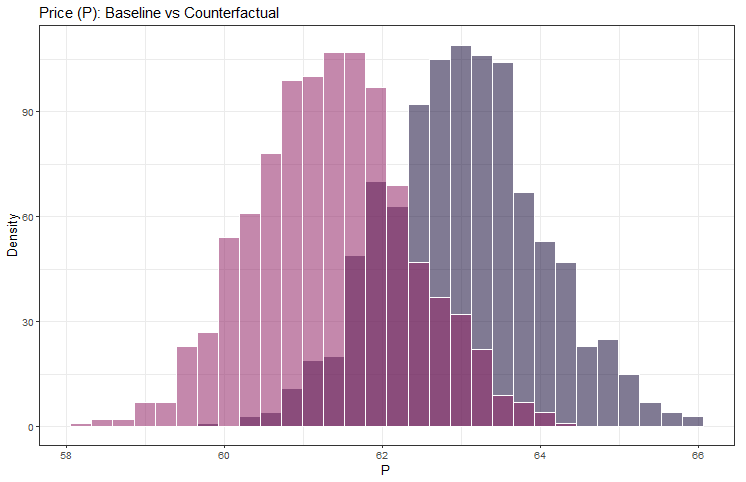
\includegraphics[width=\linewidth]{2.png}
    \end{subfigure}
    \begin{subfigure}{0.49\textwidth}
        \centering
        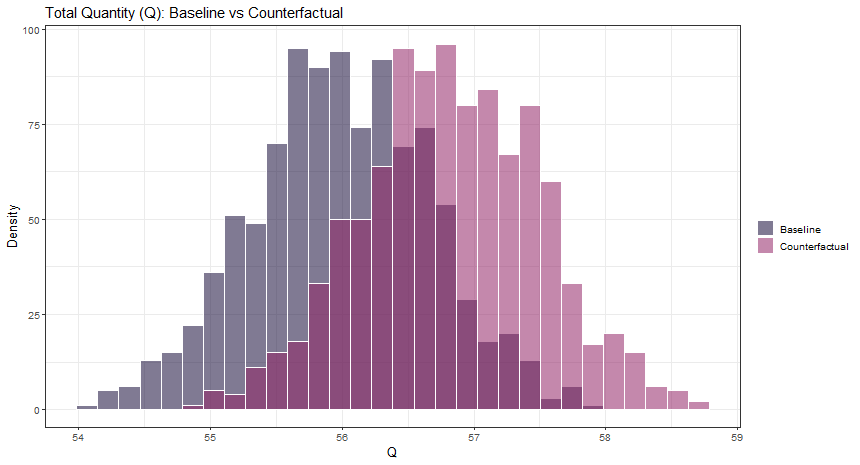
\includegraphics[width=\linewidth]{3.png}
    \end{subfigure}
\end{figure}


\begin{figure}[h]
\centering
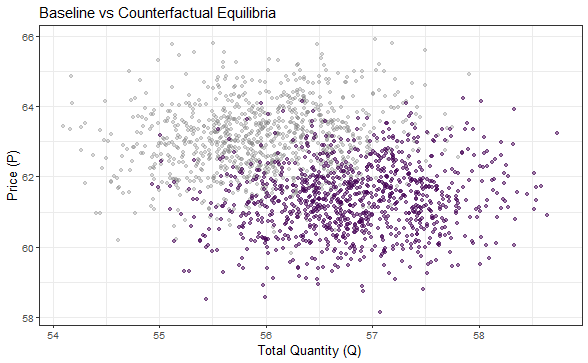
\includegraphics[width=\linewidth]{4.png}
\end{figure}


\end{document}